\section{Arbeitsjournal}
Da ich das ganze Projekt in einer Subversion umgebung aufgesetzt habe, kann man unter http://code.google.com/p/stuve/updates/list nachlesen, wann ich was abgeschlossen habe.\\
 Trotzdem wäre es auch noch spannend, wenn man sehen könnte für was man als Entwickler am meisten Zeit benötigt. Deshalb habe ich ein paar Diagrammer erstellt, die das aufzeigen sollten.
\subsection{OOP}
Zuerst einen Blick nur auf die OOP, also die Umsetzung des Projektes.\\
Die Angaben sind in Stunden gehalten.
\begin{figure}[ht]
\begin{center}
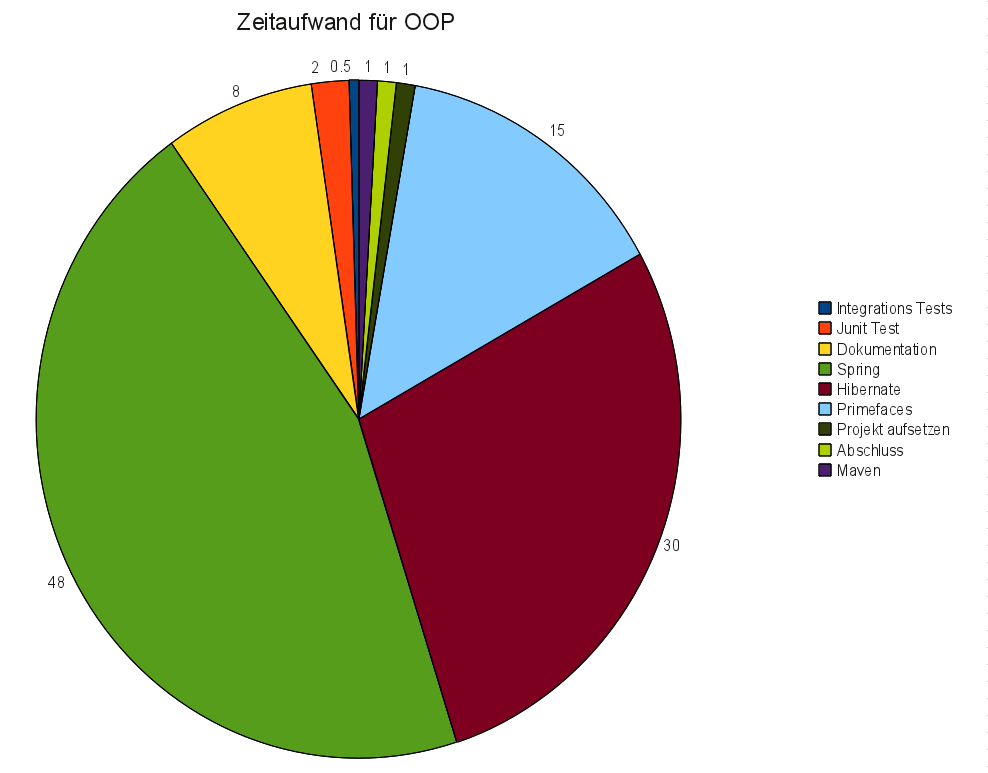
\includegraphics[width=15cm]{images/OOP.png}
\caption{Zeitaufwand für OOP}
\end{center}
\end{figure}
\\
Was ganz klar herausspringt ist die Zeit, die ich mit Spring verbracht habe. Es hat sich aber ganz sicher gelohnt, denn mit Hilfe von Spring ist das Zusammenspiel von Service-Klassen zu Dao-Klassen extrem einfach. Bzw. man muss sich jetzt gar nicht darum kümmern.\\
Auch ein grosser Teil, geht an das Framework Hibernate. Hier habe ich vorallem ein ausprobiert was ist wenn ich es so mache oder so.\\
Mit Primeface habe ich mich auch viel befasst. Jedoch reichte auch die Zeit am Schluss nicht, um sich dort noch weiter zu vertiefen.\\
Einen grossen Aufwand machte auch noch die Dokumentation.\\[2ex]
Man sieht also dass ich für das Projekt, am meisten Zeit in das Lernen von den Frameworks gesteckt habe. Ich denke aber, dass sich diese Zeit extrem gelohnt hat. Denn durch die Frameworks wird mit beim Programmieren einiges ersparrt und ich kann dann dort wieder Zeit sparen.

\subsection{Ganzes Projekt}
\begin{figure}[ht]
\begin{center}
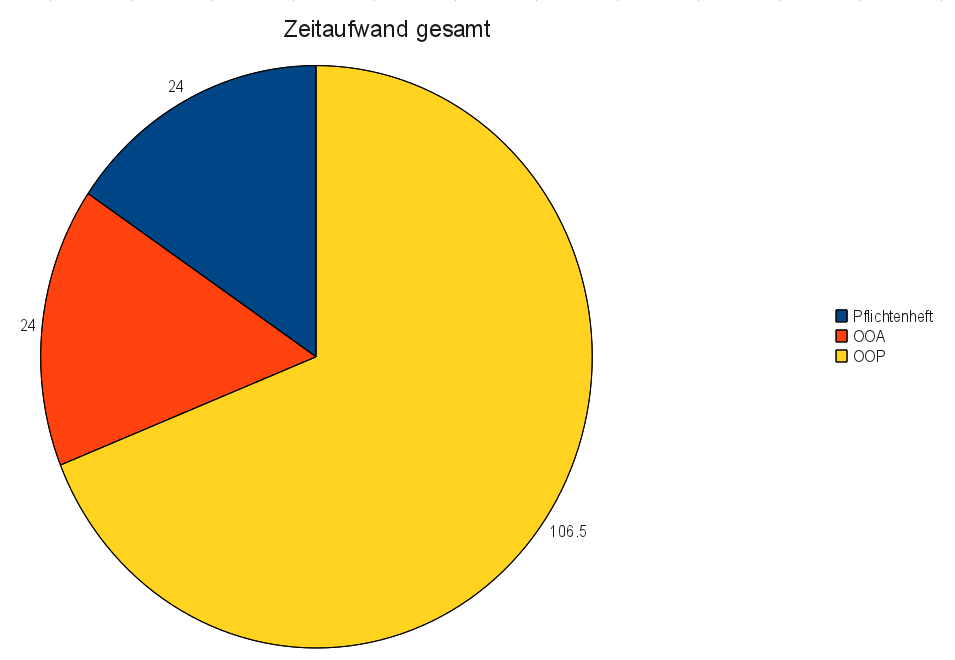
\includegraphics[width=15cm]{images/projekt_gsam.png}
\caption{Zeitaufwand für das ganze Projekt}
\end{center}
\end{figure}
Was mich auch noch wunder nahm, wie sieht es eigentlich aus, wenn man das ganze Projekt anschaut. Von der Plannung bis zur Durchführung. \\
Für die OOP wurde am meisten Zeit beansprucht. Man darf aber nicht vergessen, dass hier sehr viel Zeit ins Studium von den verschiedenen Frameworks gesteckt wurde. Müsste ich nochmal so ein Projekt machen, wäre dort die Zeit extrem viel weniger.
\clearpage
